\documentclass[10pt,a4paper,oneside]{book}

\usepackage[T1]{fontenc}
\usepackage[portuguese]{babel}
\usepackage[utf8]{inputenc}
\usepackage{amsmath}
\usepackage{color}
\usepackage{amsfonts}
\usepackage[pdfborder={0 0 0},
	    plainpages=false,
	    pdfpagelabels,
	    pdftex,
        pdfauthor={Frederico Mendonça Passos de Lopes e Gonçalves},
        pdftitle={Miavita Developed Software User Manual},
        pdfsubject={Miavita User Manual},
        pdfproducer={pdflatex with hyperref},
        pdfcreator={pdflatex}]{hyperref}
\usepackage{simplemargins}
\usepackage{graphicx}
\usepackage{listings}

\setallmargins{1in}

\title{\textbf{Manual de Software Desenvolvido para o Miavita}}
\author{Frederico Gonçalves\\MEIC-T, 57843\\\href{mailto:frederico.lopes.goncalves@gmail.com}{frederico.lopes.goncalves@gmail.com}}
\date{\today}

\begin{document}
\maketitle

\tableofcontents

\chapter{Preparação do Sistema}

\section{Cross-compilation}

Esta secção demonstra como compilar programas para o ARM a partir de uma outra plataforma (cross-compiling). As vantagens são óbvias. O processo de compilação é muito mais rápido e por vezes não é de todo possível compilar código no ARM, como é o caso dos módulos para o kernel. Isto deve-se ao facto de a \emph{source} do kernel não estar presente no ARM, pois é demasiado grande.

De modo a poder compilar código para o ARM noutra plataforma é necessário uma versão do \emph{gcc} preparada para tal. Esta pode ser obtida no site \emph{ftp} da TS - \href{ftp://ftp.embeddedarm.com/ts-arm-sbc/ts-7500-linux/cross-toolchains/}{ftp://ftp.embeddedarm.com/ts-arm-sbc/ts-7500-linux/cross-toolchains/}. O pacote não traz apenas uma versão diferente do \emph{gcc}, traz também uma versão diferente da \emph{libc}, denominada \emph{uclibc} (micro libc) e ainda um conjunto de ferramentas associadas ao processo de compilação. A \emph{uclibc} destingue-se da \emph{libc} por ser muito mais pequena e estar desenhada para correr em sistemas embebidos. É perfeitamente normal que funções presentes na \emph{libc} não se encontrem na \emph{uclibc}. Por esta razão é extremamente recomendável usar a \emph{cross-toolchains} mais recente possível, de modo a trazer a versão mais actual da \emph{uclibc}.

Uma vez feito o download basta desarquivar o ficheiro para um local onde este fique permanentemente. Por exemplo:

\begin{center}
{\tt tar xvzf crosstool-linux-gcc.tar.gz  -C $\sim$}
\end{center}

Os binários para compilar programas encontram-se em:

\begin{center}
{\tt $\sim$/arm-unknown-linux-gnu/bin/}
\end{center}

Embora seja possível usar o compilador especificando o caminho todo, é bastante mais produtivo adicioná-lo à \emph{PATH}, de modo a poder ser chamado de qualquer lado. Para tornar o processo automático é também recomendável inserir o próximo comando no ficheiro {\tt $\sim$/.bashrc}.

\begin{center}
{\tt export PATH=\$PATH:/home/fred/arm-unknown-linux-gnu/bin/}
\end{center}

Se tudo correr bem, o seguinte comando deve produzir a versão do \emph{gcc} para o ARM.

\begin{center}
{\tt arm-unknown-linux-gnu-gcc --version}
\end{center}

Estes são todos os passos necessários para preparar o sistema para compilar programas para o ARM. Para usar o compilador basta fazê-lo da mesma forma que usaríamos o \emph{gcc}. Como por exemplo:

\begin{center}
{\tt arm-unknown-linux-gnu-gcc -o exec main.c}
\end{center}

Para compilar o kernel também é necessário usar este novo compilador, mas neste caso é necessário alterar a Makefile do kernel e substituir a variável \emph{CROSS\_COMPILE} por \emph{CROSS\_COMPILE=arm-unknown-linux-gnu-} (Note-se que não é suposto ter \emph{gcc} no final).

\section{Código do Projecto}

Esta secção explica como obter o código do projecto. Todo o código desenvolvido para o projecto encontra-se no \emph{github}, precisamente em \href{https://github.com/cnm/mia\_vita}{https://github.com/cnm/mia\_vita}. 

Uma vez feito o \emph{clone} do repositório é possível observar as seguintes directorias principais:

\begin{flushleft}
  {\tt
    kernel\_sender/\\
    interruption/\\
    rt2501/\\
    rt3070/\\
    fred\_framework/
  }
\end{flushleft}

Estas directorias são as que contém a maior parte do código desenvolvido e/ou modificado e é nelas que o resto do manual se foca.

De notar que embora o comando {\tt git branch -a} mostre vários \emph{branches} remotos, o código principal encontra-se no \emph{master}.

\chapter{Código}

 Esta secção explica todo o código desenvolvido. Mais precisamente, descreve quais as funções de cada componente, como compilá-los e correr.

  \section{Kernel Sender e Programa Servidor}
  
  A directoria {\tt kernel\_sender/} contém o código que prepara os pacotes e envia-os para o nó \emph{sink}. Este por sua vez deverá ter uma instância do programa que recebe os dados a correr. Este programa encontra-se em {\tt kernel\_sender/user}.

  \subsubsection{Kernel Sender}\label{sec:sender}

    O programa que envia os dados (\emph{sender\_kthread.ko}) opera em \emph{kernel land}. A principal razão para este facto prende-se com a forma como as amostras são recolhidas do ADC. Estas são recolhidas por um módulo de kernel (\emph{int\_mod.ko} localizado em {\tt interruption/}) criado pelo João Trindade que preenche um \emph{buffer} com tais amostras e as temporiza. Seria possível ler este \emph{buffer} a partir de um programa em \emph{user land}, contudo isto traria um \emph{overhead} indesejável, pelo que optou-se por fazer o programa cliente também em \emph{kernel land}.

    Como seria de esperar, o módulo que envia os dados depende do módulo que recolhe as amostras. Como tal, este último tem de ser compilado primeiro. Na directoria {\tt kernel\_sender/} encontra-se um \emph{script} com o nome \emph{compile.bash}. Este \emph{script} trata de compilar tanto o módulo \emph{int\_mod.ko} como o módulo \emph{sender\_kthread.ko}, resolvendo todas as dependências.

    Quando o módulo \emph{sender\_kthread.ko} foi desenvolvido, o protocol de sincronização estava em fase de testes. O objectivo dos testes era comparar o atraso dado por dispositivos GPS, face ao atraso medido pelo protocolo. Por esta razão, várias zonas do código encontram-se circunscritas por {\tt \#ifdef \_\_GPS\_\_ ... \#endif}. Para que o código seja compilado para os testes com GPS basta passar ao compilador a \emph{flag} {\tt -D\_\_GPS\_\_}. Como isto trata-se de um módulo de kernel, é preciso abrir a Makefile e adicionar a linha:

    \begin{center}
      {\tt EXTRA\_CFLAGS+=-D\_\_GPS\_\_}
    \end{center}

    Note-se que ao compilar este módulo para correr os testes com GPS, é necessário também compilar o código do driver (Secção \ref{sec:driver}) e o programa que recebe os dados com a mesma \emph{flag}.

    É extremamente importante perceber que esta \emph{flag} não faz com que o valor de criação do pacote passe a ser medido pelo GPS. Apenas prepara o código para os testes com GPS. O valor de criação do pacote continua a ser medido pelo protocolo de sincronização. Para alterar o código de modo a usar o valor do GPS como tempo de criação do pacote é necessário alterar as zonas marcadas com comentários no código.
    (TODO Fred Marca com comentários e faz listagem dos ficheiros sff)

    É ainda possível compilar o módulo com informação de \emph{debug} que é emitida para {\tt /var/log/syslog}. Neste caso é necessária a \emph{flag} {\tt -DDBG}.

    O módulo \emph{sender\_kthread.ko} tem uma funcionalidade muito simples. Limita-se a criar uma \emph{thread}, que por sua vez abre um socket e de X em X tempo vai lendo N amostras do \emph{buffer} de amostras em \emph{int\_mod.ko} (ficheiro source: proc\_entry.c). Por cada amostra é criado um pacote e os dados são enviados para o \emph{sink}. É preciso especificar pelo menos o IP do \emph{sink} e o do próprio nó. Isto pode ser feito em \emph{runtime}. Para saber todos os parâmetros de um módulo basta usar o comando:

    \begin{flushleft}
      {\tt 
        modinfo sender\_kthread.ko\\\hfill\\
        filename:       ./sender\_kthread.ko\\
        description:    This module spawns a thread which reads the buffer exported by João and
                        sends samples accross the network.\\
        author:         Frederico Gonçalves, [frederico.lopes.goncalves@gmail.com]\\
        license:        GPL v2\\
        depends:        int\_mod\\
        vermagic:       2.6.24.4 mod\_unload ARMv4 \\
        parm:           bind\_ip:This is the ip which the kernel thread will bind to. Default is localhost. (charp)\\
        parm:           sink\_ip:This is the sink ip. Default is localhost. (charp)\\
        parm:           sport:This is the UDP port which the sender thread will bind to. Default is 57843. (ushort)\\
        parm:           sink\_port:This is the sink UDP port. Default is 57843. (ushort)\\
        parm:           node\_id:This is the identifier of the node running this thread. Defaults to 0. (ushort)\\
        parm:           read\_t:The sleep time for reading the buffer. (uint)
      }
    \end{flushleft}

    Especificar parametros para um módulo é bastante simples. Como exemplo:

    \begin{flushleft}
      {\tt insmod sender\_kthread.ko bind\_ip=''192.168.2.123'' sink\_ip=''192.168.2.1''}
    \end{flushleft}

    Por fim é preciso ter em conta a especificação do pacote de dados (Secção \ref{sec:packet_specification}). Todos os campos são enviados em \emph{network byte order}, que é \emph{Big Endian}. Os processadores ARM podem funcionar tanto em \emph{Little Endian}, como em \emph{Big Endian}. Infelizmente, os processadores das placas TS-7500 funcionam em \emph{Little Endian}, pelo que os dados têm de ser convertidos antes de serem enviados. Para tipos de dados alinhados, isto é, inteiros de 16, 32 e 64 bits o kernel já fornece funções que fazem a conversão. Contudo, cada amostra tem 24 bits, pelo que não existe nenhuma função que faça a conversão por nós. Esta foi então implementada na função \emph{read\_nsamples} localizada no ficheiro \emph{interruption/proc\_entry.c}. O modo como foi implementada foi pensado para ser o mais rápido possível, evitando ciclos. Contudo é preciso ter especial cuidado com o seguinte. Esta conversão depende de dois grande factores:

    \begin{enumerate}
    \item Assume que o ARM trata os dados como \emph{Little Endian}. Se por alguma razão o \emph{hardware} mudar, é preciso verificar se esta conversão está a ser feita correctamente.
    \item Assume que o código no ficheiro \emph{interruption/fpga.c} lê as amostras de uma forma especifica. Se este código mudar, é necessário verificar se a conversão contínua a ser bem feita. Por outras palavras, o código da função \emph{read\_nsamples} é extremamente dependente do código do ficheiro \emph{interruption/fpga.c}.
    \end{enumerate}

    \subsubsection{Programa Servidor}
    
    Na directoria {\tt kernel\_sender/user} encontra-se o programa que recebe os dados do módulo {\tt sender\_kthread.ko}. Para compilar o programa basta usar a Makefile dentro da directoria. A Makefile define a variável {\tt CC}, que é usada para determinar qual o compilador a usar. Para compilar o programa para o ARM, basta alterar esta variável para reflectir o caminho para o \emph{cross-compiler}. Por exemplo:

    \begin{flushleft}
      {\tt make CC=arm-unknown-linux-gnu-gcc}
    \end{flushleft}

    Tal como os módulos do kernel, este código também pode ser compilado para ser usado nos testes com GPS. Neste caso é preciso adicionar à \emph{flag} {\tt CFLAGS} a opção {\tt -D\_\_GPS\_\_}, dentro da Makefile. O \emph{output} do programa são dois ficheiros, um em formato binário e outro em formato json (ver Secção \ref{sec:packet_specification}). É preciso ter em conta que quando são feitos os testes com GPS, o campo \emph{timestamp} reflecte o atraso medido pelo protocolo de sincronização e um campo adicional (\emph{gps\_us}) reflecte o atraso medido pelo GPS. O primeiro encontra-se em nanosegundos e o último em microsegundos.

    Os pacotes são escritos para o ficheiro binário tal e qual como chegam ao socket. Contudo, antes de serem escritos para o formato json, são convertidos para a \emph{byte order} do CPU. Tanto o ficheiro binário, como o ficheiro json são rotativos. Os pacotes são escritos para um ficheiro A. Na próxima escrita, o ficheiro A é movido para um ficheiro B e rescrito com os novos pacotes. Todos os nomes e tamanhos do ficheiro são configuráveis em \emph{runtime}:

    \begin{flushleft}
      ./main -h\\\hfill\\
      Usage: ./main [-i <interface>] [-p <listen\_on\_port>] [-b <output\_binary\_file>] [-j <output\_json\_file>] [-o <moved\_file\_prefix>]\\
      -i Interface name on which the program will listen. Default is eth0\\
      -p UDP port on which the program will listen. Default is 57843\\
      -b Name of the binary file to where the data is going to be written. Default is miavita.bin\\
      -j Name of the json file to where the data is going to be written. Default is miavita.json\\
      -t Test the program against GPS time. Make sure to compile this program with -D\_\_GPS\_\_.\\
      -o Output file prefix when the file is moved by log rotation. Default is miavita\_old.\\
      -c Buffer capacity expressed in terms of number of packets. Default is 100.
    \end{flushleft}

    Na altura da escrita deste manual, a interface gráfica para o utilizador necessitava de ler os ficheiros json com os pacotes ordenados por \emph{timestamp}. Como tal, o programa que recebe os dados faz \emph{buffering} de X pacotes e antes de os escrever ordena-os. O mecanismo de \emph{buffering} e rotação dos ficheiros encontra-se implementado no ficheiro {\tt list.c}. Embora todos os X pacotes sejam ordenados, apenas $\frac{X}{2}$ são escritos para os ficheiros. Isto serve para evitar ao máximo que um pacote atrasado fique desordenado nos ficheiros.
    
\section{RT2501 - Driver Modificado}\label{sec:driver}

O driver fornecido pela Ralink foi modificado para sincronizar os pacotes de acordo com o algoritmo descrito na minha tese. A principal diferença é que o código actual faz tudo ao nível do driver e não necessita da \emph{framework} de interceptores.

A ideia é conseguir interceptar os pacotes enviados no último momento possível. Neste caso, trata-se da função que submete o pacote ao controlador de USB (função {\tt RTUSBBulkOutDataPacket} no ficheiro {\tt rtusb\_bulk.c}). Por outro lado, também é necessário interceptar os pacotes recebidos o mais cedo possível. Neste caso, trata-se da \emph{callback} chamada pelo controlador de USB (função {\tt REPORT\_ETHERNET\_FRAME\_TO\_LLC} no ficheiro {\tt rtusb\_data.c}).

As funções que sincronizam os pacotes enviados e recebidos encontram-se no ficheiro {\tt sync\_proto.c}. É preciso notar que as funções que submetem pacotes ao controlador de USB e recebem pacotes do mesmo, são chamadas para todos os pacotes enviados e recebidos. Por esta razão é preciso impedir que o \emph{driver} tente sincronizar pacotes que nada têm haver com o módulo \emph{sender\_kthread.ko}. Como por exemplo pacotes ARP. Para este efeito pensou-se no conceito de filtros, muito semelhante ao modo como funcionam as \emph{iptables}. Neste caso, são definidos um conjunto de filtros que indicam qual o tráfego a sincronizar. Estes filtros encontram-se implementados no ficheiro {\tt filter\_chains.c}. Quando nenhum filtro é especificado, nenhum pacote é sincronizado. Contudo, é possível definir filtros para sincronizar, por exemplo, todo o tráfego gerado na porta 57843 pelo IP 192.168.0.123. O driver assume que quando um pacote passa nas especificações de um filtro tem o formato especificado no capitulo \ref{sec:packet_specification}.

Uma vez mais, se todos os outros componentes foram compilados para os testes com GPS, este também o deverá ser (Adicionar a \emph{flag} {\tt EXTRA\_CFLAGS+=-D\_\_GPS\_\_} à Makefile).

Os filtros podem ser definidos em \emph{runtime}. Para tal, o driver implementa uma entrada \emph{proc} ({\tt /proc/synch\_filters}) que recebe dados num dado formato e cria os filtros apropriados. Na directoria {\tt rt2501/sources/Module/user} encontram-se dois programas que tratam de criar e remover filtros. É necessário compilar os programas para o ARM, pelo que a Makefile deve reflectir o compilador apropriado. Opcionalmente pode-se ainda correr o comando {\tt make install} para que os comandos de filtros fiquem instalados no sistema. De modo a saber como usar os comandos, basta corrê-los sem argumentos.

O comando que remove filtros recebe o identificador do filtro a remover. É possível saber este identificador através do comando:

\begin{flushleft}
  {\tt cat /proc/synch\_filters}
\end{flushleft}

Este comando imprime também todas as especificações dos filtros criados. É preciso ter atenção que todos os nós por onde o pacote passa têm de ter os mesmos filtros criados de modo a que o protocolo funcione.

\section{Kernel Modificado}\label{sec:kernel}

O kernel fornecido pela TS foi modificado de modo a conter mais duas \emph{system calls}. Uma é usada para fazer \emph{set} ao tempo do GPS e outro é usada para obter este tempo. O ficheiro {\tt README.rst} no repositório do miavita, explica como adicionar \emph{system calls} ao ARM. Este kernel pode ser obtido fazendo:

\begin{center}
{\tt git clone https://github.com/cnm/ts7500\_kernel}
\end{center}

O tempo do GPS é mantido em duas variáveis dentro do kernel (\_miavita\_elapsed\_secs, \_miavita\_elapsed\_usecs). Uma mantém os segundos dados pelo GPS a outra mantém os microsegundos dados pelo ARM. Não é possível obter menos do que um segundo do GPS, pelo que os microsegundos do ARM são usados. Assume-se que dentro de um segundo o \emph{drift} do cristal do ARM não é significativo.

Ambas as variáveis têm 64 bits e são \emph{signed}. Encontram-se dentro da directoria {\tt ipc} dentro das \emph{sources} do kernel, no ficheiro {\tt miavita\_syscall.c}. A função {\tt pulse\_miavita\_xtime} é chamada pelo módulo \emph{int\_mod.c} (Secção \ref{sec:sender}) a cada interrupção dada pelo PPS do GPS. Isto garante que a variável que mantém os segundos tem a mesma precisão que o PPS do GPS, que é cerca de 50 nanosegundos.

O ficheiro {\tt miavita\_syscall.c} implementa não só as \emph{system calls} criadas, mas também o modo como outros módulos podem interagir com as variáveis que mantém o tempo do GPS. Para que outros módulos usem tais funções é necessário que incluam o ficheiro {\tt miavita\_xtime.h} ({\tt \#include <linux/miavita\_xtime.h>}). Dentro do repositório do miavita, existe uma directoria denominada {\tt interruption/}, onde está um ficheiro com o nome {\tt fpga.c}. Este ficheiro contém exemplos de como estas variáveis podem ser usadas.

\chapter{Especificação do Pacote de Dados}\label{sec:packet_specification}

  \section{Binário}

	Esta secção mostra como os dados são mantidos no ficheiro binário. A figura \ref{fig:packet} mostra a estrutura de cada pacote.
	
	 \begin{figure}[h!]
   	  \centering
   	  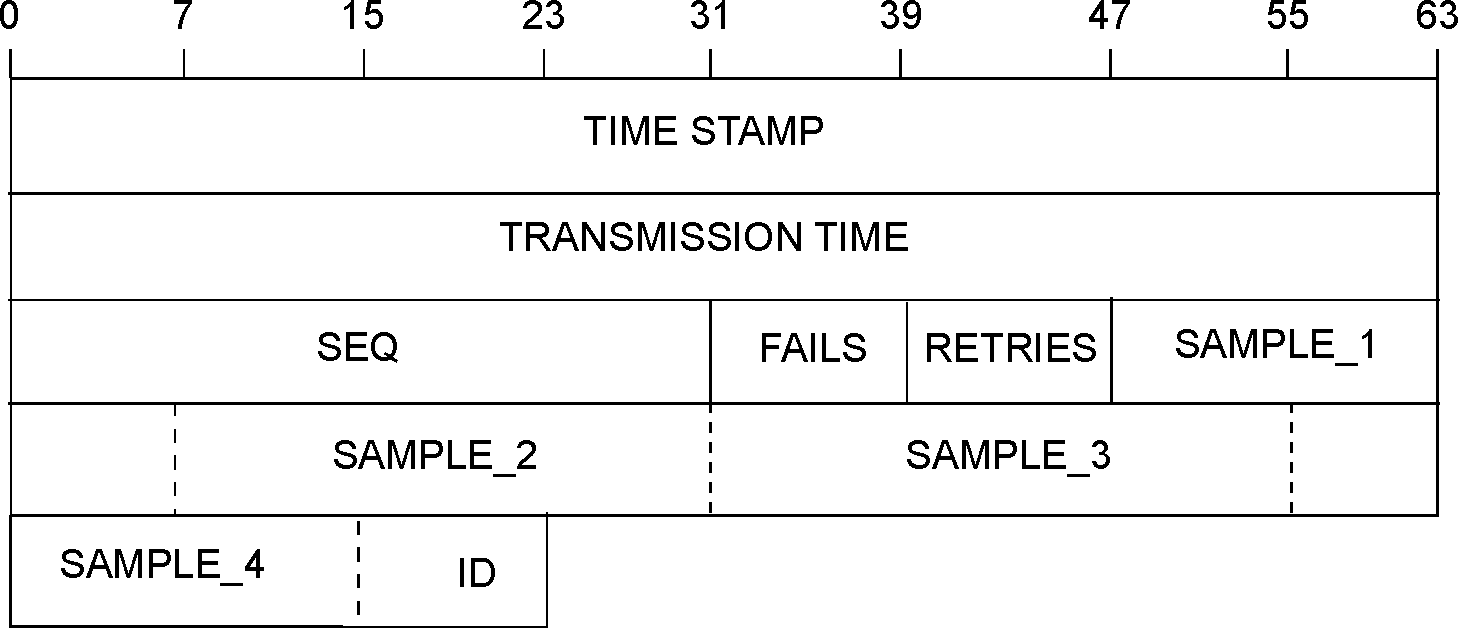
\includegraphics[width=0.7\textwidth]{packet.pdf}
	  \caption{Pacote de dados.}
   	  \label{fig:packet}
 	\end{figure}

	Cada campo do pacote é descrito da seguinte forma, quando transmitido na rede:

 \begin{description}
   \item[Time stamp]\hfill\\
   	O primeiro campo do pacote é usado para um valor de tempo, com 64 bits, \emph{signed} e transmitido em \emph{Big Endian}. Este campo representa o tempo de criação do pacote, ou o tempo que passou desde que o pacote foi criado.
   \item[Air time estimation]\hfill\\
   	O segundo campo no pacote é usado para um valor de tempo, com 64 bits, \emph{signed} e transmitido em \emph{Big Endian}. Este campo representa o tempo de transmissão estimado pelo driver.
   \item[Sequence number]\hfill\\
   	O terceiro campo no pacote é usado para um valor de um número de sequência, com 32 bits, \emph{unsigned} e transmitido em \emph{Big Endian}.
   \item[Fails]\hfill\\
         O quarto campo no pacote é usado para fornecer à aplicação o número de falhas que ocorreram desde o último pacote recebido. Este campo pode incluir falhas de todos os pacotes, não só aqueles que pertencem à aplicação.
   \item[Retries]\hfill\\
         O quinto campo no pacote é usado para fornecer à aplicação o número de retransmissões que ocorreram desde o último pacote recebido. Este campo pode incluir retransmissões de todos os pacotes, não só aqueles que pertencem à aplicação.
   \item[Samples]\hfill\\
     O sexto campo é usado para guardar 4 amostras retiradas do Geophone, com 24 bits, \emph{signed} e transmitidas em \emph{Big Endian}.
    \item[Node Identifier]\hfill\\
	O último campo identifica o nó da rede.
 \end{description}

  \section{ASCII}
  
  	Esta secção fornece informação sobre o formato ascii usado para representar os pacotes. O ficheiro de \emph{output} tem um formato JSON, onde as chaves são compostas por {\tt <identificador do nó>:<número de sequência do pacote>}. O seguinte é um exemplo de um ficheiro com o formato descrito.

  \lstinputlisting[language=Python]{packet.py}  
  
  
\chapter{Como Usar os Componentes}

	Esta secção demonstra como correr e instalar cada componente de modo a ter um caso de uso do miavita. Por agora o cartão tem de poder ser escrito. Em primeiro lugar é necessário ter o kernel descrito na secção \ref{sec:kernel} preparado para \emph{flashar} na placa ARM. Este é o procedimento que utilizei:
	
	\begin{enumerate}
		\item No meu computador dentro da pasta que contém o kernel executo {\tt make modules modules\_install zImage}.
		\item Insiro  o cartão do ARM no meu computador.
		\item Apago a pasta {\tt /lib/modules/2.6.24.4/} do cartão, executando\\ {\tt rm -r /media/<particao4>/lib/modules/2.6.24.4/}.
		\item Copio os novos módulos para dentro do cartão, executando\\ {\tt cp -r /lib/modules/2.6.24.4/ /media/<particao4>/lib/modules/}.
		\item Ponho o novo kernel na partição dois do cartão SD, executando\\ {\tt dd if=arch/arm/boot/zImage of=/dev/sdb2} (Atenção que o caminho do \emph{output} pode variar).
		\item Como normalmente quero que o kernel na \emph{flash} seja o mesmo do cartão, faço logo uma cópia para dentro do cartão SD de modo a poder \emph{flashá-lo} mais tarde. Executo \\{\tt dd if=/dev/sdb2 of=/media/<particao4>/root/zImage.dd}
		\item Não esquecer de desmontar o cartão - {\tt umount /media/*}
		\item Ponho o cartão numa placa ARM e em geral uso uma \emph{board} de desenvolvimento para concluir o procedimento.
		\item Ponho a \emph{board} a \emph{bootar} pelo cartão SD.
		\item Em primeiro lugar, faço o \emph{flash} do novo kernel:
			\begin{flushleft}
				{\tt spiflashctl -W 4095 -z 512 -k part1 -i zImage.dd}
			\end{flushleft}
		\item Após concluído, é preciso criar as dependências dos módulos, executando {\tt depmod}.
		\item Por fim, é preciso fazer \emph{reboot} à placa.
	\end{enumerate}

	Em segundo lugar, é preciso pôr o módulo rt73.ko na placa. Este passo pode ser intercalado com o anterior, mas assim fica mais explícito o que é necessário fazer:
	
	\begin{enumerate}
		\item Copio o módulo normalmente para a pasta\\
		 {\tt /lib/modules/2.6.24.4/kernel/drivers/net/wireless/rt2xx0/}.
		\item Após concluído, é preciso criar as dependências dos módulos outra vez, executando {\tt depmod}.
		\item Por fim, é preciso fazer \emph{reboot} à placa.
	\end{enumerate}
	
	Terceiro passo consiste em copiar os programas e módulos para dentro do ARM de modo a poder usá-los.

	\begin{enumerate}
		\item No meu computador, compilo todos os programas e módulos com o \emph{cross-compiler} para o ARM. Isto inclui, programa utilizador que recebe os dados, programas que criam e removem os filtros, o módulo \emph{int\_mod.ko} e o módulo \emph{sender\_kthread.ko}.
		\item Copio todos os componentes para dentro do cartão SD. Em específico, copio os programas {\tt mkfilter} e {\tt rmfilter} para dentro da pasta {\tt /usr/bin/}. De notar que não vale de muito ter o módulo \emph{sender\_kthread.ko} e o programa que recebe os dados na mesma placa.
	\end{enumerate}
	
	\textbf{A partir daqui o sistema está pronto para ser usado. É necessário colocar o cartão em \emph{read-only}}.
	
	Para iniciar um caso de uso do miavita, é necessário matar alguns processos. O seguinte comando deve ser efectuado a cada \emph{boot} da placa:
	
	\begin{center}
		{\tt kill \$(pgrep xuartctl); kill \$(pgrep daqctl);  kill \$(pgrep dioctl); kill -9 \$(pgrep logsave); kill \$(pgrep ts7500ctl); sleep 2; ts7500ctl --autofeed 3; sleep 5; kill \$(pgrep ts7500ctl);}
	\end{center}
	
	De seguida é necessário inserir os módulos para dar início ao programa que recolhe e envia amostras para o sink. De notar que o driver rt2501 modificado já foi inserido automaticamente quando se inseriu a pen wifi.
	
	\begin{enumerate}
		\item Inserir o módulo que recolhe amostras: {\tt insmod int\_mod.ko}
		\item Inserir o módulo que envia as amostras: {\tt insmod  sender\_kthread.ko bind-ip=''<IP da placa wifi>''  sink-ip=''<ip da placa wifi do sink>''}
	\end{enumerate}
	
	Por fim, basta colocar no sink o programa que recebe os dados a correr:
	
	\begin{center}
		{\tt ./main -i rausbwifi}
	\end{center}
	
	A partir deste ponto as placas estarão a enviar dados para o sink e este a recebê-los. Caso seja necessário testar o protocolo com GPS é preciso compilar os componentes com a \emph{flag} {\tt -D\_\_GPS\_\_} e antes de inserir qualquer módulo é preciso inicializar as variáveis no kernel (Secção \ref{sec:kernel}). Para tal é preciso usar o programa {\tt init\_counter} dentro da directoria {\tt kernel\_sender/user/}. Compila-se com:
        
        \begin{center}
          {\tt make CC=arm-unknown-linux-gnu-gcc init\_counter}
        \end{center}
	
        A seguir é preciso correr o programa antes de inserir qualquer módulo. É preciso ter em conta que o programa inicializa o programa {\tt xuartctl}, que tem de ser terminado após o programa {\tt init\_counter} terminar. É ainda preciso ter atenção que o programa tenta abrir o \emph{device} do GPS mais comum que as placas criam ({\tt /dev/pts/1}). É possível especificar outro \emph{device} com a \emph{flag} {\tt -d}. Contudo, o nome do \emph{device} só é conhecido após o programa {\tt xuartctl} ter inicializado. Por esta razão, se o \emph{device} for outro é preciso matar o {\tt xuartctl} antes de correr outra vez o programa {\tt init\_counter}.

\chapter{Framework de Interceptores}

  Dentro da directoria {\tt fred\_framework/} encontra-se o código correspondenete à framework de interceptores. A ideia de tal framework é criar uma estrutura base onde outros módulos do kernel (Interceptores) se possam registar e interceptar o tráfego em cada nó. Por exemplo, a agregação de pacotes realizado no projecto miavita é feita através de dois interceptores. Um é responsável por interceptar o tráfego e agregá-lo, enquanto que outro é responsável por desagregá-lo.

  A framework trabalha por cima da API de Netfilters do kernel. Assim que o módulo da framework é inserido no kernel, são registados 5 hooks (Um para cada ponto de intercepção fornecidos pelo Netfilters - Post routing, local in, etc.). Cada interceptor regista-se na framework para poder interceptar o tráfego desejado. Para que cada interceptor só esteja ciente do tráfego que realmente precisa de interceptar, a framework fornece um mecanismo que permite filtrar tráfego não desejado. Isto é atingido através de umas estruturas denominadas \textbf{regras}. As regras são simplesmente um conjunto de \textbf{filtros}. Os filtros são estruturas que possuem um conjunto de especificações e um ponto de interacção. Por exemplo, uma regra para agregar tráfego ao nível da rede e aplicação, com destino à porta 57843 e ip 192.168.0.1 iria criar uma regra com dois filtros. Um filtro iria actuar no ponto de intercepção \emph{local out} e o outro no ponto de intercepção \emph{post routing}. Ambos os filtros iriam conter uma especificação que iria informar a framework que todo o tráfego com aquele destino deve ser interceptado pelo interceptor de agregação.
  
  Em suma, a framework de interceptores permite o registo de um ou mais interceptores que definem regras para que possam interceptar um subconjunto dos pacotes que passam no nó.

  Ao nível da implementação, as regras são criadas através de um comando user level que escreve para um ficheiro proc. Este comando denomina-se \emph{mkrule}. De forma semelhante existe um comando para eleminar regras - \emph{rmrule}. No ficheiro {\tt README.rst} na pasta {\tt fred\_framework} está descrito como usar estes comandos. Existe ainda a explicação de como usar o comando {\tt emsg} para determinar a mensagem de erro associada a um código de erro.
  
  \section{Interceptor de agregação} 

   Como o nome indica, este interceptor é responsável por agregar o tráfego que sai de um dado nó. No ficheiro {\tt README.rst} na pasta {\tt fred\_framework} descreve como usar este interceptor. Este documento explica como o protocolo funciona.

   \subsection{Nível Aplicação}
   
    Na realidade, este tipo de agregação deveria chamar-se agregação ao nível transporte, pois os pacotes são agregados de acordo com informação no header UDP. Contudo, por razões ``históricas'' continou-se a chamar agregação ao nível da aplicação.

    Quando um pacote a ser agregado é interceptado pelo protocolo de agregação este procederá da seguinte forma: 

    \begin{enumerate}
      \item Se não existir um buffer associado ao destino desse, o protocolo cria um.
      \item O pacote é inserido no buffer.
      \item Se o buffer ficar cheio, um pacote agregado é construído e enviado para o destino.
    \end{enumerate}

    Neste tipo de agregação os pacotes são agregados da seguinte forma:

    {\tt
      |IP header | UDP N | UDP N - 1| ... | UDP 0 |
    }

    Isto significa que os pacotes são enviados por ordem inversa. O header IP é criado pelo protocolo de agregação na altura do seu envio. Este header leva informação no seu campo de protocolo a informar que este é um pacote agregado ao nível da aplicação.
    
    É preciso ter em atenção que o protocolo cria uma thread que de X em X tempos irá fazer \emph{flush} a todos os buffers de agregação com pacotes pendentes.

   \subsection{Nível Rede}
   
    Este tipo de agregação segue o mesmo processo do que aquele descrito na agregação ao nível da aplicação. Contudo, o pacote agregado passa a ter este aspecto:

    {\tt
      |IP header | IP N | IP N - 1| ... | IP 0 |
    }

    Isto significa que os pacotes agregados são agora pacotes IP completos e podem portanto vir de origens diferentes. A mesma thread que faz \emph{flush} aos pacotes agregados ao nível aplicacional, também o faz aos pacotes agregados ao nível da rede. O primeiro header IP é criado pelo protocolo de agregação, mas deste vez o campo do protocolo indica que este pacote é agregado ao nível da rede. 

  \section{Interceptor de desagregação} 

   O interceptor de desagregação limita-se a desagregar os pacotes, simplesmente olhando para o tipo de protocolo que vem no header IP e procedendo à desagregação ao nível rede ou aplicacional.

   Contudo, devido ao facto de os pacotes virem por ordem inversa é necessário um pequeno passo, para que estes sejam entregues pela ordem certa. Para isto, existe um buffer global com tamanho suficiente para conter o máximo de pacotes possível dentro de uma MTU, onde os pacotes são temporariamente postos. Este buffer denomina-se \emph{scatter\_buffer}.

   A ideia é a seguinte.
   
   \begin{enumerate}
    \item O pacote agregado é percorrido apenas uma vez.
    \item Apontadores para cada pacote são guardados dentro deste buffer, do fim para o princípio.
    \item No final, o buffer é percorrido e os pacotes são entregues pela ordem correcta.
   \end{enumerate}
\end{document}
